\documentclass[12pt,english]{beamer}
\usepackage[mathletters]{ucs}
\usepackage[utf8x]{inputenc}
\usepackage{babel}
\usepackage{xcolor}
\usepackage{listings}
\usepackage{textcomp}
\usepackage[noBBpl]{mathpazo}
\usepackage{courier}
\usepackage{fancyvrb}
\usepackage{amsmath}
\usepackage{amssymb}
\usepackage{url}

\usecolortheme{crane}
\usefonttheme{serif}

\usepackage{tikz}
\usetikzlibrary{arrows,calc,shapes,chains}

\newcommand{\K}{\mathbb{K}}  % Biot-Savart kernel
\newcommand{\R}{\mathbb{R}}  % set of real numbers
\renewcommand{\vec}{\mathbf}
\newcommand{\x}{\vec x}      % position
\newcommand{\vel}{\vec u}    % velocity
\DeclareMathOperator{\divergence}{div}
\DeclareMathOperator{\curl}{curl}
\DeclareMathOperator{\supp}{supp}
\providecommand{\abs}[1]{\lvert#1\rvert}
\providecommand{\norm}[1]{\lVert#1\rVert}
\newcommand{\pd}[2]{\frac{\partial #1}{\partial #2}}
\newcommand{\md}[2]{\frac{D#1}{D#2}}
\newcommand{\od}[2]{\frac{d#1}{d#2}}

\title{GPU-accelerated simulation of a Lamb--Oseen vortex
using 2-D Vortex Methods}
\author{Roberto Bonvallet}
\date{March 28th, 2011}

\begin{document}
  \begin{frame}
    \maketitle
  \end{frame}

  \begin{frame}
    \frametitle{Fluid Dynamics}
    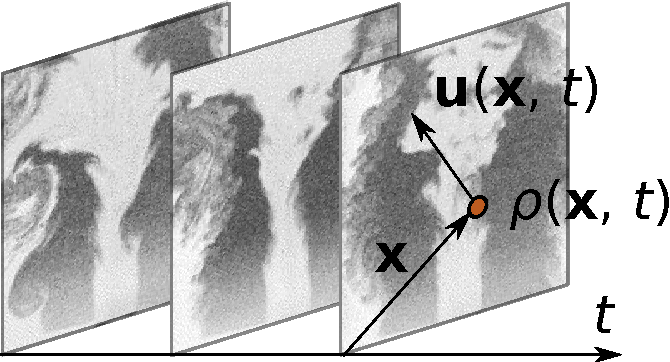
\includegraphics{fluid1.pdf}
  \end{frame}

  \begin{frame}
    \frametitle{Eulerian methods}
    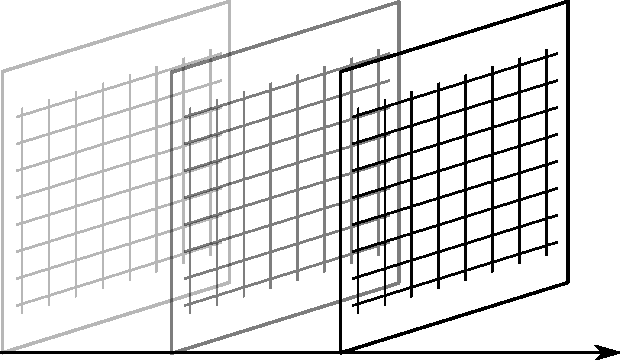
\includegraphics{fluid2.pdf}
  \end{frame}

  \begin{frame}
    \frametitle{Lagrangian methods}
    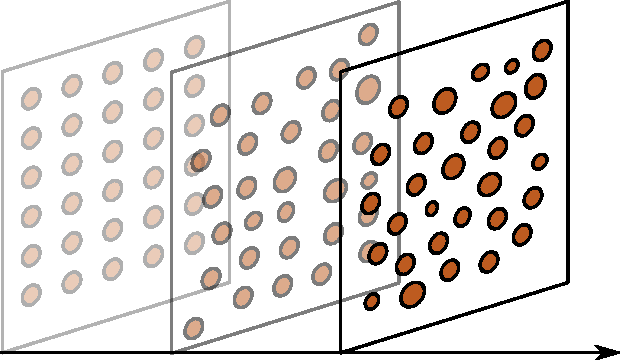
\includegraphics{fluid3.pdf}
  \end{frame}

  \begin{frame}
    \frametitle{Fluid equations in Eulerian coordinates}
    \begin{itemize}
      \item Continuity equation:
        \begin{equation}
          \pd{ρ}{t} + ∇\cdot(ρ\vel) = 0
        \end{equation}
      \item Navier-Stokes equations:
        \begin{equation}
          ρ\left(\pd{\vel}{t} + \vel\cdot∇\vel\right) = -∇p + μ\,Δ\vel + \vec{f}
        \end{equation}
    \end{itemize}
  \end{frame}

  \begin{frame}
    \frametitle{Fluid equations in Lagrangian coordinates}
    \begin{itemize}
      \item Continuity equation:
        \begin{equation}
          \md{ρ}{t} = -ρ\divergence\vel
        \end{equation}
      \item Navier-Stokes equations:
        \begin{equation}
          ρ\md{\vel}{t} = -∇p + μ\,Δ\vel + \vec{f}
        \end{equation}
    \end{itemize}
  \end{frame}

  \begin{frame}
    \frametitle{2-D Vortex Methods}
    \begin{itemize}
      \item Incompressible flow:
        \begin{itemize}
          \item  \(∇\cdot\vel = 0\);
          \item continuity equation reduces to \(\displaystyle\md{ρ}{t} = 0\).
        \end{itemize}
      \item Velocity-vorticity formulation of N-S eqs.:
        \begin{align}
          ρ\md{\vel}{t} &= -∇p + μ\,Δ\vel \\
          ρ\md{ω}{t}    &= μ\,Δω \\
          \md{ω}{t}    &= ν\,Δω
        \end{align}
    \end{itemize}
  \end{frame}

  \begin{frame}
    \frametitle{2-D Vortex Methods}
    \begin{align}
      \md{ω}{t} &= ν\,Δω \\
      \divergence\vel &= 0 \\
      \curl\vel &= \mathbold\omega \\
      ω(\,\cdot\,, 0) &= ω_0
    \end{align}
  \end{frame}

  \begin{frame}
    \frametitle{Recovery of velocity}
    \begin{itemize}
      \item Velocity field recovered by solving Poisson's equation:
        \begin{equation}
          \left.
          \begin{split}
            \divergence\vel &= 0 \\
            \curl\vel &= \mathbold\omega
          \end{split}
          \right\}\;\Longrightarrow\;
          Δ\vel = -\curl\mathbold\omega
        \end{equation}
      \item Biot-Savart law:
        \begin{align}
          \vel(\x, t) &=
            \int\bigl(\curl\vec{G}\bigr)(\x - \x')\,ω(\x', t)\,d\x' \\
          \vel &= \K * ω,
            \quad\text{where \(\textstyle\K(x, y) = -\frac{1}{2π\norm{\x}}(-y, x)\)}
        \end{align}
    \end{itemize}
  \end{frame}

  \begin{frame}
    \frametitle{Vortex Point Method}
    \begin{itemize}
      \item Domain discretized as a set of particles.
      \item Approximation of the vorticity field:
        \begin{equation}
          ω^h(x, t) \approx\sum_p α_p δ\bigl(\x - \x^h_p(t)\bigr)
        \end{equation}
      \item Velocity restored by Biot-Savart law
    \end{itemize}
  \end{frame}

  \begin{frame}
    \frametitle{Vortex Blob Method}
    \begin{itemize}
      \item Smooth cutoff function \(ζ\) such that \(\int ζ(\x)\,d\x = 1\).
      \item Mollified particle: \(ζ_ε(\x) = ε^{-2} ζ(\x/ε)\).
      \item Mollified kernel:   \(\K_ε = \K * ζ_ε\).
      \item Numerical method:
        \begin{align}
          \od{\x^h_p}{t} &= \vel^h(\x^t_p, t) \\
          \od{ω^h_p}{t}    &= ν\,Δω^h_p
        \end{align}
        with \(\vel^h = \K_ε * ω^h\).
    \end{itemize}
  \end{frame}

\end{document}
